\documentclass[12pt]{article}
\usepackage[utf8]{inputenc}
\usepackage[brazil]{babel}
\usepackage{graphicx}
\usepackage{amsmath}
\usepackage{listings}
\usepackage{color}
\usepackage{caption}
\usepackage{geometry}
\geometry{a4paper, margin=2.5cm}

\definecolor{codegray}{rgb}{0.5,0.5,0.5}
\definecolor{codepurple}{rgb}{0.58,0,0.82}

\lstset{
  language=[x86masm]Assembler,
  basicstyle=\ttfamily\footnotesize,
  keywordstyle=\color{blue},
  commentstyle=\color{codegray},
  stringstyle=\color{codepurple},
  numbers=left,
  numberstyle=\tiny\color{codegray},
  stepnumber=1,
  numbersep=5pt,
  showstringspaces=false,
  breaklines=true,
  breakatwhitespace=false,
  tabsize=2
}

\title{Projeto de Processador REDUX-V}
\author{Pietro Comin}
\date{\today}

\begin{document}

\maketitle

\begin{abstract}
Este relatório documenta o projeto do processador REDUX-V, abordando sua arquitetura, conjunto de instruções, componentes principais como a ULA e a memória de controle, além da justificativa para instruções estendidas adicionadas. O relatório também contém um exemplo de código Assembly otimizado com essas instruções.
\end{abstract}

\section{Introdução}

O processador REDUX-V é uma arquitetura simples desenvolvida com fins didáticos, incorporando instruções básicas e capacidade de extensão via instruções adicionais. O projeto envolve a criação de um datapath, unidade de controle e suporte a instruções imediatas e saltos condicionais.

\section{Conjunto de Instruções Base}

A arquitetura REDUX-V suporta um conjunto enxuto de instruções, como:

\begin{itemize}
  \item Operações lógicas: \texttt{and}, \texttt{or}, \texttt{not}, \texttt{xor}
  \item Operações aritméticas: \texttt{add}, \texttt{sub}, \texttt{addi}
  \item Controle de fluxo: \texttt{ji} (jump immediate), \texttt{brzr} (branch if zero)
  \item Manipulação de registradores e memória: \texttt{load}, \texttt{store}, \texttt{move}
\end{itemize}

\section{Datapath do Processador}

\begin{figure}[h!]
\centering
\includegraphics[width=0.9\textwidth]{/images/datapath.png}
\caption{Datapath do processador REDUX-V}
\label{fig:datapath}
\end{figure}

O datapath define o caminho de dados percorrido durante a execução de uma instrução. Ele inclui componentes como o banco de registradores, a ULA, multiplexadores, unidade de controle e memória de dados.

\section{Projeto da ULA}

\begin{figure}[h!]
\centering
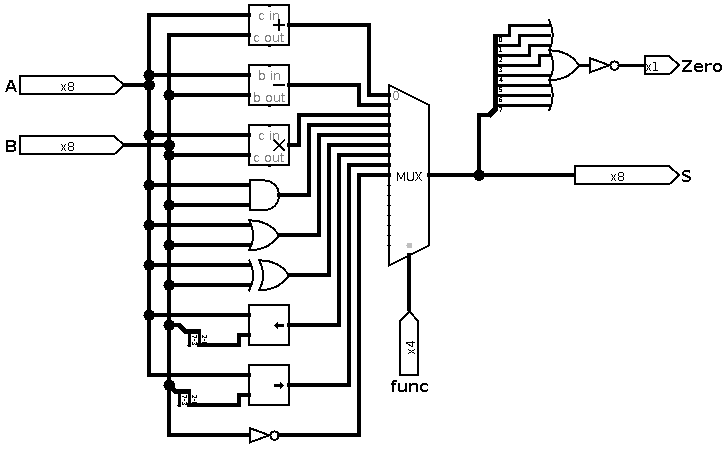
\includegraphics[width=0.75\textwidth]{/images/ALU.png}
\caption{Diagrama interno da ULA}
\label{fig:ula}
\end{figure}

A ULA é responsável por executar as operações lógicas, aritméticas e de deslocamento da arquitetura REDUX-V. Ela recebe dois operandos e um código de operação, realizando o processamento e enviando o resultado ao banco de registradores ou à memória.

\subsection{Operações Suportadas}
\begin{itemize}
  \item Operações lógicas: \texttt{not}, \texttt{and}, \texttt{or}, \texttt{xor}
  \item Operações aritméticas: \texttt{add}, \texttt{sub}, \texttt{addi}, \texttt{muli}
  \item Deslocamentos: \texttt{slr}, \texttt{srr}
  \item Comparações: implícitas no controle de fluxo (\texttt{brzr})
\end{itemize}

\subsection{Controle da ULA}
O código de operação que define o comportamento da ULA é fornecido pela memória de controle, a partir do opcode decodificado da instrução atual.

\section{Memória de Controle}

A memória de controle foi projetada para fornecer os sinais necessários à execução de cada instrução, com base no opcode correspondente. Ela determina os sinais de controle para os multiplexadores, leitura e escrita de registradores, operação da ULA e controle de fluxo (como atualização do PC).

\begin{figure}[h!]
\centering
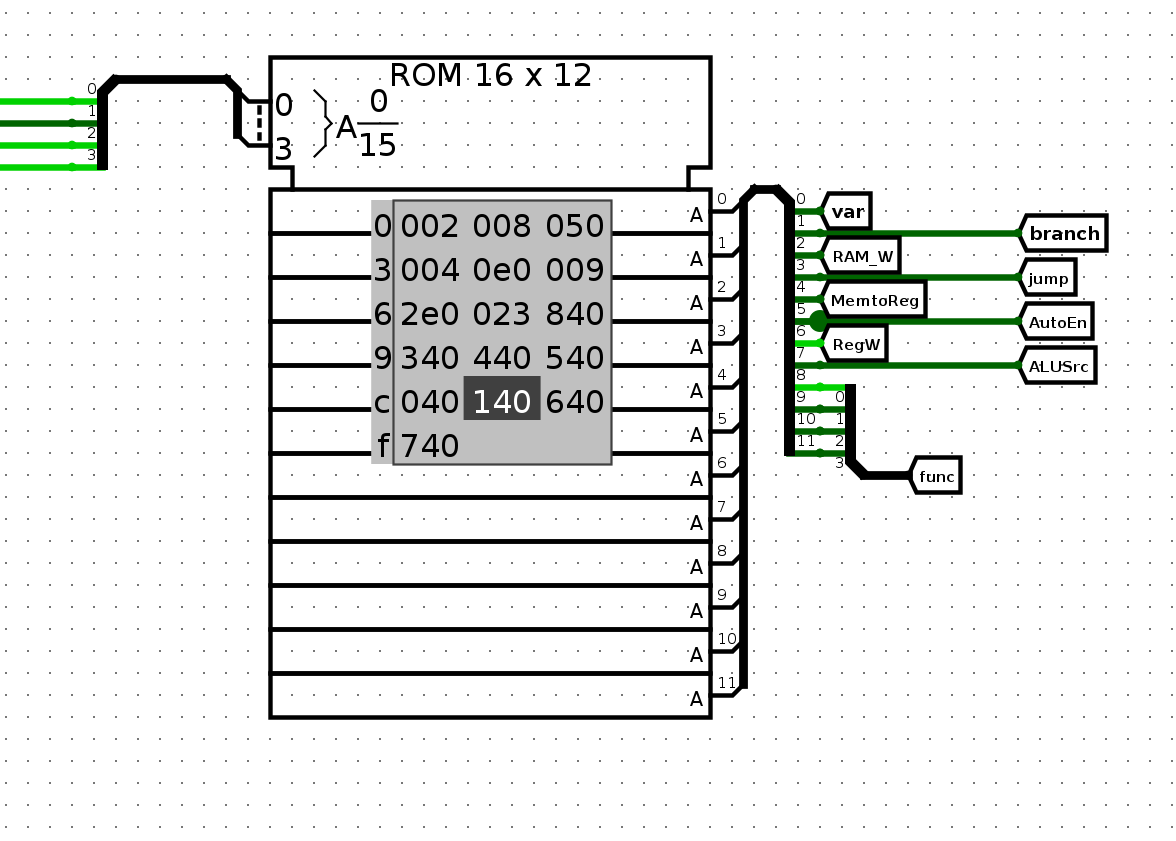
\includegraphics[width=0.85\textwidth]{/images/controll_memory.png}
\caption{Diagrama da memória de controle do processador REDUX-V}
\label{fig:memoria_controle}
\end{figure}

\section{Justificativa das Instruções Adicionais}

As três instruções estendidas adicionadas à arquitetura (\texttt{jien}, \texttt{muli} e \texttt{brzrue}) visam ampliar a capacidade da linguagem de máquina e tornar os programas mais enxutos e expressivos.

\begin{itemize}
  \item \textbf{jien} (Jump Immediate Extended Negative): permite saltos para trás mais longos do que o \texttt{ji}. Ideal para loops e estruturas de repetição.
  \item \textbf{muli} (Multiplication Immediate): substitui múltiplas instruções \texttt{addi} por uma única operação de multiplicação com imediato.
  \item \textbf{brzrue} (Branch on Zero Unsigned Extended): permite saltos condicionais longos para frente, o que facilita implementações mais complexas com bifurcações.
\end{itemize}

\subsection{Exemplo de Código com Instruções Estendidas}

\begin{lstlisting}
; Programa que calcula um valor, aplica salto positivo e negativo
loop:
brzrue 2      ; PC = PC + 12 (se r[0] == 0, salta para fim_loop)
... (11 instrucoes)
jien 1        ; PC = PC - 11 (salto para loop)

fim_loop:
...
\end{lstlisting}

Essas instruções contribuem para a legibilidade e eficiência do código Assembly por aumentar o range de saltos.

\section{Conclusão}

O projeto do processador REDUX-V evidenciou os princípios fundamentais da arquitetura de computadores, incluindo o funcionamento de uma ULA, memória de controle e fluxo de dados via datapath. As instruções adicionais propostas aumentaram a flexibilidade da linguagem e a expressividade dos programas escritos para essa arquitetura.

\end{document}
